%%%%%%%%%%%%%%%%%%%%%%%%%%%%%%%%%%%%%%%%%
% a0poster Portrait Poster
% LaTeX Template
% Version 1.0 (22/06/13)
%
% The a0poster class was created by:
% Gerlinde Kettl and Matthias Weiser (tex@kettl.de)
% 
% This template has been downloaded from:
% http://www.LaTeXTemplates.com
%
% License:
% CC BY-NC-SA 3.0 (http://creativecommons.org/licenses/by-nc-sa/3.0/)
%
%%%%%%%%%%%%%%%%%%%%%%%%%%%%%%%%%%%%%%%%%

%----------------------------------------------------------------------------------------
%	PACKAGES AND OTHER DOCUMENT CONFIGURATIONS
%----------------------------------------------------------------------------------------

\documentclass[a0,portrait]{a0poster}

\usepackage{multicol} % This is so we can have multiple columns of text side-by-side
\columnsep=100pt % This is the amount of white space between the columns in the poster
\columnseprule=3pt % This is the thickness of the black line between the columns in the poster

\usepackage[svgnames]{xcolor} % Specify colors by their 'svgnames', for a full list of all colors available see here: http://www.latextemplates.com/svgnames-colors

\usepackage{times} % Use the times font
%\usepackage{palatino} % Uncomment to use the Palatino font

\usepackage{graphicx} % Required for including images
\graphicspath{{figures/}} % Location of the graphics files
\usepackage{booktabs} % Top and bottom rules for table
\usepackage[font=small,labelfont=bf]{caption} % Required for specifying captions to tables and figures
\usepackage{amsfonts, amsmath, amsthm, amssymb} % For math fonts, symbols and environments
\usepackage{wrapfig} % Allows wrapping text around tables and figures

\newtheorem{definition}{Definition}

\begin{document}

%----------------------------------------------------------------------------------------
%	POSTER HEADER 
%----------------------------------------------------------------------------------------

% The header is divided into two boxes:
% The first is 75% wide and houses the title, subtitle, names, university/organization and contact information
% The second is 25% wide and houses a logo for your university/organization or a photo of you
% The widths of these boxes can be easily edited to accommodate your content as you see fit

\begin{minipage}[b]{0.75\linewidth}
\veryHuge \color{NavyBlue} \textbf{Expanders} \color{Black}\\ % Title
\Huge\textit{From Network reliability to $K$-theory}\\[2cm] % Subtitle
\huge \textbf{Cl\'ement Dell'Aiera \\under supervision of Herv\'e Oyono-Oyono}\\[0.5cm] % Author(s)
\huge Universit\'e de Lorraine\\[0.4cm] % University/organization
\Large \texttt{clement.dell-aiera@univ-lorraine.fr} \\
\end{minipage}
%
\begin{minipage}[b]{0.25\linewidth}

\includegraphics[width=20cm]{IECL.png}\\
\end{minipage}

\vspace{1cm} % A bit of extra whitespace between the header and poster content

%----------------------------------------------------------------------------------------

\begin{multicols}{2} % This is how many columns your poster will be broken into, a portrait poster is generally split into 2 columns

%----------------------------------------------------------------------------------------
%	ABSTRACT
%----------------------------------------------------------------------------------------

\color{Navy} % Navy color for the abstract

%\begin{abstract}
%\end{abstract}

%----------------------------------------------------------------------------------------
%	INTRODUCTION
%----------------------------------------------------------------------------------------

%\color{SaddleBrown} % SaddleBrown color for the introduction

\section*{Introduction}

Building networks, for instance the Internet network, one wants reliabilty with respect to link or node failure, and maintain a low cost. It turns out that a class of graph, called expanders, are very sparse as well as very well connected. Sparsity means that there are very few links compared to the number of vertices (or node), and well connectedness is a property fostering robustness.\\

We propose to explain how we could measure well-connectedness, and describe expanders.

%----------------------------------------------------------------------------------------
%	OBJECTIVES
%----------------------------------------------------------------------------------------
 
\color{DarkSlateGray} % DarkSlateGray color for the rest of the content

\section*{Random walk and Laplacian}

A graph is made of vertices and edges between them. We will only consider finite graphs, i.e. graphs with a finite number of vertices. The first figure shows a family of graphs, which could represent networks for instance, or people being friends with one another, or, for geneticists, genes interacting with one another.\\

\begin{center}\vspace{1cm}
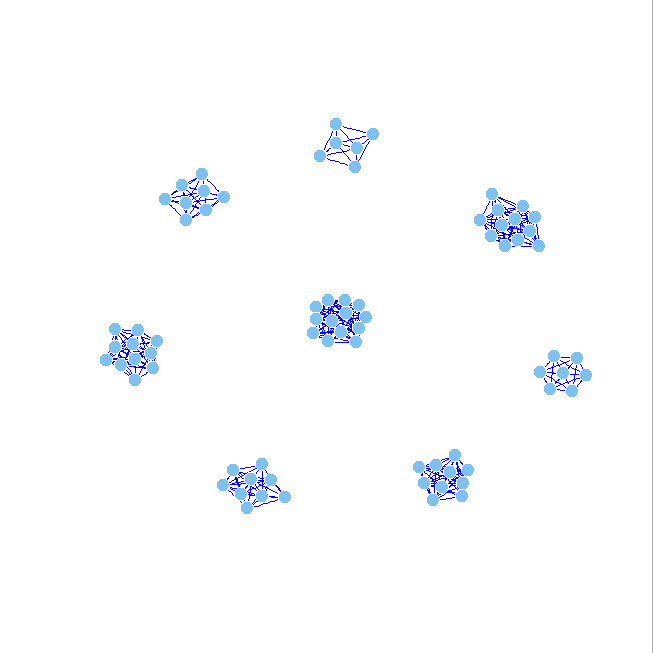
\includegraphics[width=0.9\linewidth]{Graphs5}
\captionof{figure}{\color{Green} A family of graphs}
\end{center}\vspace{1cm}

You would like to be able to measure how connected a graph is. A natural way to do so is to look at uniform random walk on the graph. The more the connectedness, the easier it is to get from one point to another. For examples, we say that expanders are very-well connected because the random walk converges very quickly to the uniform distribution, that is randomly exploring the graph, you only need a few steps to being close to choosing randomly your destination on the entire graph.\\

The random walk on a graph is defined as follow :\\
\begin{enumerate}
\item Choose a vertex
\item A each step, choose the following vertex uniformly amongst the neighbours of your current vertex.\\
\end{enumerate}

Mathematically, a graph is a a couple $(V,E)$, $V$ being the set of vertices, and $E\subset V\times V$. Define, for $v\in V$, the set of neighbours of $v$ as $N_v=\{w\in V / (v,w)\in E\}$ and the degree of $x$ as $deg(x)=|N_x|$.The random walk is a Markov chain defined by:\\
\begin{enumerate}
\item $X_0=v_0$
\item $X_{n+1}|X_n\sim \mathcal U_{N_{X_n}}$. \\
\end{enumerate}

A natural operator associated to random walk is the Laplacian $\Delta \in \mathcal L(l^2(V))$.
\[(\Delta f) (x) = f(x) - \frac{1}{deg(x)}\sum_{y\in N_x} f(y) .\] 

It turns out that $\Delta$ is a positive operator, and if the graph is connected, its kernel consists of constant functions. So its ordered spectrum $\lambda_0\leq \lambda_1<\lambda_2...$ always satisfies $\lambda_0=0$, and $\lambda_1$ measures in a sense the connectedness of the graph.\\

The second figure shows what the Laplacian looks like for the family of graphs of the previous picture.\\

\begin{center}\vspace{1cm}
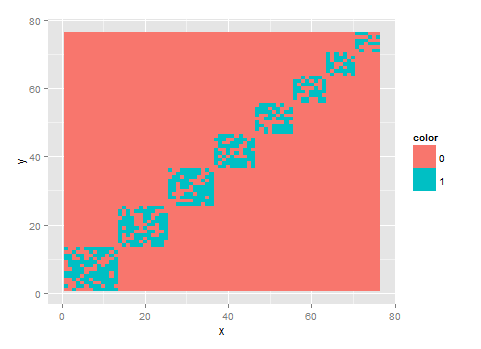
\includegraphics[width=0.9\linewidth]{Laplacian}
\captionof{figure}{\color{Green} Laplacian of the family}
\end{center}\vspace{1cm}

\section*{Expanders}

\begin{definition}
An expander is a family $X=(X_j)_j$ of finite graphs $(X_j,E_j)$ such that 
\begin{itemize}
\item[$\bullet$] $\lim_{j}|X_j|=\infty$
\item[$\bullet$] the degree of the graphs is constant : $\exists k, deg(X_j)=k,\forall j$,
\item[$\bullet$] the second eigenvalue of the Laplacian is bounded above : $sp(\Delta_j)\subset \{0\}\cup [\epsilon,1]$.
\end{itemize}
\end{definition}
When speaking of expanders, we often confuse them with the metric space consisting of the coarse disjoint union of all the graphs, which is just a metric space with the distance induced by the length on the graph when restricted to one of the graph, and such that $\lim_{j+k\rightarrow \infty}d(X_j,X_k)$.\\

An interesting property of expanders is that they cannot be coarsely embed into Hilbert space. Recall that we say that a metric space $(X,d_X)$ coarsely embeds into Hilbert space if there exists two increasing functions $\rho_{+/-}: \mathbb R_+\rightarrow \mathbb R_+$ and a map $\phi : X\rightarrow H$ such that :
\[\rho_-(d_X(x,y))\leq ||\phi(x)-\phi(y)||_H \leq \rho_+(d_X(x,y))\quad,\forall x,y\in X,\]
where $H$ is the separable Hilbert space.\\

One way to construct expanders is to give yourself a finitely generated group $\Gamma$ which is residually finite w.r.t. $\mathcal N=\{\Gamma_j\}$, a nested family of normal subgroups $\Gamma_0 > \Gamma_1>...$ with trivial intersection, and to form the coarse disjoint union of the metric spaces $\Gamma/\Gamma_j$,
\[X_{\mathcal N}(\Gamma)=\sqcup_j \Gamma/\Gamma_j.\]
If $\Gamma$ has property $\tau$ w.r.t. $\mathcal N$, i.e. if the trivial representation is isolated in the topological space of representation factorizing through $\Gamma/\Gamma_j$, then $X_{\mathcal N}(\Gamma)$ is an expander. In particular, Kazdhan's property (T) implies proerty $\tau$, so that property (T) groups satisfy this obstruction. For example, you can take $SL(n,\mathbb Z)$ for $n\geq 3$. \\ 

%----------------------------------------------------------------------------------------
%	CONCLUSIONS
%----------------------------------------------------------------------------------------

\color{SaddleBrown} % SaddleBrown color for the conclusions to make them stand out

\section*{Conclusions}

Guoliang Yu proved \cite{yu} that every space $X$ that coarsely embeds into Hilbert space satisfies the coarse Baum-Connes conjecture, which gives an algorithm to compute the $K$-theory of the Roe algebra of $X$. Now expanders cannot be coarsely embedded into Hilbert space, so that we did not know how to compute $K_*(C^*X)$ for an expander $X$. The first example of such a result was achieved by Herv\'e Oyono-Oyono and Guoliang Yu in \cite{oyono} where they computed $K(C^*_{max}X)$ for expanders coming from the previous example $X_{\mathcal N}(\Gamma)$. This result was generalized to spaces which admits a coarse fibered embedding into Hilbert space by Martin Finn-Sell in \cite{finn}. \\

My work focus on applying controlled $K$-theory, a refined version of $K$-theory keeping track of propagation when the underlying $C^*$-algebra is filtered, to these problems. In particular, we defined a controlled version of the Baum-Connes conjecture for groupoids, which allows us to state similar results that of \cite{finn} but in a quantitative way. \\

\color{DarkSlateGray} % Set the color back to DarkSlateGray for the rest of the content

%----------------------------------------------------------------------------------------
%	FORTHCOMING RESEARCH
%----------------------------------------------------------------------------------------

 %----------------------------------------------------------------------------------------
%	REFERENCES
%----------------------------------------------------------------------------------------

\nocite{*} % Print all references regardless of whether they were cited in the poster or not
\bibliographystyle{plain} % Plain referencing style
\bibliography{biblio} % Use the example bibliography file sample.bib

%----------------------------------------------------------------------------------------
%	ACKNOWLEDGEMENTS
%----------------------------------------------------------------------------------------

\section*{Acknowledgements}

I would like to thank Herv\'e Oyono-Oyono for reading the first drafts of this poster. 
The template used for the poster was created by Gerlinde Kettl and Matthias Weiser and can be freely downloaded at
http://www.latextemplates.com/template/a0poster-portrait-poster.

%----------------------------------------------------------------------------------------

\end{multicols}
\end{document}
